% Aufgabe f: Klirrfaktor
% U_2_f: 0.005303300858899106 in V
% f_2_f: 0.14907119849998599
% k: 0.035575623676894264
\nocite{anleitungV302}
\section{Auswertung}
\label{sec:Auswertung}
Im Folgenden werden die Mittelwerte mit 
$$\bar{x} = \frac{1}{n} \cdot \sum_{i = 1}^{n}x_i$$ bestimmt. $n$ ist die Anzahl der Daten und $x_i$ die einzelnen Daten.
Mit der Gaußschen Fehlerfortpflanzung
$$\Delta f = \sqrt{\sum_{i = 1}^{n} \left( \frac{\partial f}{\partial x_i} \right)^2 \cdot \left(\Delta x_i \right)^2}$$
werden die Messunischerheiten ausgerechnet, wenn eine Größe von mehreren fehlerbehafteten Größen abhängt.
\subsection{Wheatstonesche Brücke}
\label{sec:WheatstonescheBrücke}
Zunächst wird der unbekannte Widerstand $R_{13}$ verwendet. Die verwendeten und gemessenen Widerstände sind in der Tabelle (\ref{tab:WheatstonescheBrücke_1})
aufgelistet. Der Widerstand wird mit der Gleichung (\ref{eqn:}) berechnet. Bei der Berechnung der Messunischerheiten wird der Fehler $\Delta\frac{R_3}{R_4} = 0,005 \cdot \frac{R_3}{R_4}$ verwendet. 
\begin{table}[H]
  \centering
  \caption{Widerstände der Wheatstonschen Brücke bei dem unbekannten Widerstand $R_{13}$.}
  \label{tab:WheatstonescheBrücke_1}
  \begin{tblr}{colspec={c c c | c}}
      \toprule
      $R_2\,[\unit{\ohm}]$ & $R_3\,[\unit{\ohm}]$ & $R_4\,[\unit{\ohm}]$ & $R_{13}\,[\unit{\ohm}]$\\
      \midrule
      332 &    490&     510 &   $(319,0\pm1,6)$\\
      500 &    339&     611 &   $(277,4\pm1,4)$\\
      1000&    242&     758 &   $(319,3\pm1,6)$\\   
      \bottomrule
  \end{tblr}
\end{table}
Daraus folgt der gemittelte Widerstand
$$ R_{13,\text{exp.}} = \left(305,2\pm0,9 \right)\,\unit{\ohm}\,.$$
Der theoretische Wert lautet
$$R_{13,\text{theo.}} = 319,5\,\unit{\ohm}\,.$$
In der Tabelle (\ref{tab:WheatstonescheBrücke_2}) sind die verwendeten und gemessenen Widerstände bei einer Durchführung mit dem 
unbekannten Widerstand $R_{14}$ aufgeführt. Der Widerstand $R_{14}$ berechnet sich erneut aus der Gleichung (\ref{eqn:}).
\begin{table}[H]
  \centering
  \caption{Widerstände der Wheatstonschen Brücke bei dem unbekannten Widerstand $R_{14}$.}
  \label{tab:WheatstonescheBrücke_2}
  \begin{tblr}{colspec={c c c | c}}
      \toprule
      $R_2\,[\unit{\ohm}]$ & $R_3\,[\unit{\ohm}]$ & $R_4\,[\unit{\ohm}]$ & $R_{14}\,[\unit{\ohm}]$\\
      \midrule
      332 &    732&     268&   $(906,8\pm4,5)$\\
      500 &    644&     356&   $(904,5\pm4,5)$\\
      1000&    474&     526&   $(901,1\pm4,5)$\\
      \bottomrule
  \end{tblr}
\end{table}
Aus dieser Tabelle lässt sich der gemittelte Widerstand
$$ R_{14,\text{exp.}} = \left(904,1\pm2,6 \right)\,\unit{\ohm}$$
bestimmen. Der theoretische Widerstand beträgt
$$R_{14,\text{theo.}} = 900\,\unit{\ohm}\,.$$
\subsection{Kapazitätsmessbrücke}
Bei dieser Durchführung wird wieder der relative Fehler wie im Abschnitt (\ref{sec:WheatstonescheBrücke}) benutzt. In der Tabelle (\ref{tab:Kapazitätsmessbrücke_1})
sind die verwendeten und gemessenen Kapazitäten und Widerstände der Kapazitätsmessbrücke bei den unbekannten $C_{15}$ und $R_{15}$ aufgelistet. 
Die unbekannten Werte werden mit den Gleichungen (\ref{eqn:}) und (\ref{eqn:}) bestimmt.
\begin{table}[H]
  \centering
  \caption{Kapazität und Widerstände der Kapazitätsmessbrücke bei den unbekannnten Werten $C_{15}$ und $R_{15}$.}
  \label{tab:Kapazitätsmessbrücke_1}
  \begin{tblr}{colspec={c c c c| c c}}
      \toprule
      $C_2\,[\unit{\nano\farad}]$& $R_2\,[\unit{\ohm}]$ & $R_3\,[\unit{\ohm}]$ & $R_4\,[\unit{\ohm}]$ &$C_{15}\,[\unit{\nano\farad}]$ & $R_{15}\,[\unit{\ohm}]$\\
      \midrule
      399&     500&     455&     545&   $(477,9\pm2,4)$ &  $(417,4\pm2,1)$\\
      750&     332&     576&     424&   $(552,1\pm2,8)$ &  $(451,0\pm2,3)$\\
      994&     664&     436&     564&   $(1285,8\pm6,4)$ & $(513,3\pm2,6)$\\  
      \bottomrule
  \end{tblr}
\end{table}
Die gemittelte ermittelte Kapazität lautet
$$C_{15,\text{exp.}}= \left( 771,9\pm2,5 \right)\,\unit{\nano\farad}\,.$$
Der entsprechende theoretische Wert beträgt
$$C_{15,\text{theo.}}= 652\,\unit{\nano\farad}\,.$$
Aus der Tabelle (\ref{tab:Kapazitätsmessbrücke_1}) lässt sich der gemittelte Widerstand
$$ R_{15,\text{exp.}} = \left(460,6\pm1,3\right)\,\unit{\ohm}$$
berechnen. Der theoretische Widerstand ist
$$ R_{15,\text{theo.}} = 473\,\unit{\ohm}\,.$$
Die Werte bei einer Durchführung mit den unbekannten Werten $C_{8}$ und $R_{8}$ sind in der Tabelle (\ref{tab:Kapazitätsmessbrücke_2}) aufgeführt.
$C_{8}$ und $R_{8}$ werden ebenfalls mit den Gleichungen (\ref{eqn:}) und (\ref{eqn:}) ermittelt.
\begin{table}[H]
  \centering
  \caption{Kapazität und Widerstände der Kapazitätsmessbrücke bei den unbekannnten Werten $C_{8}$ und $R_{8}$.}
  \label{tab:Kapazitätsmessbrücke_2}
  \begin{tblr}{colspec={c c c c| c c}}
      \toprule
      $C_2\,[\unit{\nano\farad}]$& $R_2\,[\unit{\ohm}]$ & $R_3\,[\unit{\ohm}]$ & $R_4\,[\unit{\ohm}]$ &$C_{8}\,[\unit{\nano\farad}]$ & $R_{8}\,[\unit{\ohm}]$\\
      \midrule
      399&     500&     551&     449&   $(325,1\pm1,6)$&  $(613,6\pm3,1)$\\
      750&     332&     667&     333&   $(374,4\pm1,9)$&  $(665,0\pm3,3)$\\
      994&     664&     525&     475&   $(899,3\pm4,5)$&  $(733,9\pm3,7)$\\  
      \bottomrule
  \end{tblr}
\end{table}
Daraus folgt die gemittelte Kapazität
$$C_{8,\text{exp.}}= \left( 533,0\pm1,7 \right)\,\unit{\nano\farad}\,.$$
Die theoretische Kapazität lautet
$$C_{8,\text{theo.}}= 294,1\,\unit{\nano\farad}\,.$$
Außerderm ergibt sich für den Widerstand 
$$R_{8,\text{exp.}} = \left( 670,8\pm1,9 \right)\,\unit{\ohm}$$
und der theoretische Widerstand beträgt
$$ R_{8,\text{theo.}} = 564\,\unit{\ohm}\,.$$
\subsection{Induktivitätsmessbrücke}
Der relative Fehler aus Abschnitt (\ref{sec:WheatstonescheBrücke}) gilt auch für diese Durchführung. Die verwendete Induktivität sowie die 
verwendeten und gemessenen Widerstände der Induktivitätsmessbrücke bei unbekannten $L_{19}$ und $R_{19}$ sind in der Tabelle (\ref{tab:Induktivitätsmessbrücke_1})
aufgelistet. Hier werden $L_{19}$ und $R_{19}$ mit den Gleichungen (\ref{eqn:}) und (\ref{eqn:}) bestimmt.
\begin{table}[H]
  \centering
  \caption{Induktivität und Widerstände der Induktivitätsmessbrücke bei den unbekannnten Werten $L_{19}$ und $R_{19}$.}
  \label{tab:Induktivitätsmessbrücke_1}
  \begin{tblr}{colspec={c c c c| c c}}
      \toprule
      $L_2\,[\unit{\milli\henry}]$& $R_2\,[\unit{\ohm}]$ & $R_3\,[\unit{\ohm}]$ & $R_4\,[\unit{\ohm}]$ &$L_{19}\,[\unit{\milli\henry}]$ & $R_{19}\,[\unit{\ohm}]$\\
      \midrule
      20,1&    1000&    126&     874&   $(139,42\pm0,70)$& $ (144,16\pm0,72)$\\
      14,6&    664 &    201&     799&   $(58,04\pm0,29)$&  $(167,04\pm0,84)$\\
      14,6&    1000&    291&     709&   $(35,57\pm0,18)$&  $(410,44\pm2,1)$\\  
      \bottomrule
  \end{tblr}
\end{table}
Aus dieser Tabelle wird die gemittelte Induktivität 
$$L_{19,\text{exp.}} = \left( 77,68\pm0,26 \right)\,\unit{\milli\henry}$$
bestimmt. Zudem beträgt der theoretische Wert der Induktivität
$$L_{19,\text{theo.}} = 26,96\,\unit{\milli\henry}\,.$$
Der gemittelte Widerstand lautet
$$R_{19,\text{exp.}} = \left( 240,50\pm0,80  \right)\,\unit{\ohm}\,.$$
Außerdem ist der theoretische Widerstand
$$ R_{19,\text{theo.}} = 108,7\,\unit{\ohm}$$ gegeben. 
Die zugehörigen Werte bei der Durchführung mit der unbekannten Induktivität $L_{16}$ und dem unbekannten Widerstand $R_{16}$
sind in der Tabelle (\ref{tab:Induktivitätsmessbrücke_2}) aufgelistet. Die unbekannten Werte werden nochmals mit den Gleichungen
(\ref{eqn:}) und (\ref{eqn:}) berechnet. 
\begin{table}[H]
  \centering
  \caption{Induktivität und Widerstände der Induktivitätsmessbrücke bei den unbekannnten Werten $L_{16}$ und $R_{16}$.}
  \label{tab:Induktivitätsmessbrücke_2}
  \begin{tblr}{colspec={c c c c| c c}}
      \toprule
      $L_2\,[\unit{\milli\henry}]$& $R_2\,[\unit{\ohm}]$ & $R_3\,[\unit{\ohm}]$ & $R_4\,[\unit{\ohm}]$ &$L_{16}\,[\unit{\milli\henry}]$ & $R_{16}\,[\unit{\ohm}]$\\
      \midrule
      20.1&    1000&    112&     888&   $(159,36\pm0,80)$&  $(126,13\pm0,63)$\\
      14.6&    664 &    85 &     915&   $(157,16\pm0,79)$&  $(61,68\pm0,31)$\\
      14.6&    1000&    83 &     917&   $(161,30\pm0,81)$&  $(90,51\pm0,45)$\\  
      \bottomrule
  \end{tblr}
\end{table}
Hieraus ergibt sich für die gemittelte Induktivität
$$L_{16,\text{exp.}} = \left( 159,30\pm0,50 \right)\,\unit{\milli\henry}$$ 
und die theoretische Induktivität beträgt
$$L_{16,\text{theo.}} = 132,71\,\unit{\milli\henry}\,.$$
Die aus der Tabelle (\ref{tab:Induktivitätsmessbrücke_2}) gemittelte Widerstand lautet
$$R_{16,\text{exp.}} = \left( 92,77\pm0,28 \right)\,\unit{\ohm}\,.$$
Der dazugehörige theoretische Widerstand ist
$$ R_{16,\text{theo.}} = 411,2\,\unit{\ohm}\,.$$ 
\subsection{Maxwell-Brücke}
In diesem Abschnitt wird wieder der gleiche relative Fehler aus Abschnitt (\ref{sec:WheatstonescheBrücke}) verwendet. Die erste Durchführung
ist erneut mit der unbekannten Induktivität $L_{19}$ und dem unbekannten $R_{19}$. Diese Werte werden mithilfe der Gleichungen (\ref{eqn:}) 
und (\ref{eqn:}) bestimmt. In der Tabelle (\ref{tab:MaxwellBrücke_1}) sind die verwendetene sowie gemessenen Widerstände, die genutzte Kapazität
und die berechneten $L_{19}$ und $R_{19}$ aufgelistet.
\begin{table}[H]
  \centering
  \caption{Induktivität und Widerstände der Maxwell-Brücke bei den unbekannnten Werten $L_{19}$ und $R_{19}$.}
  \label{tab:MaxwellBrücke_1}
  \begin{tblr}{colspec={c c c c| c c}}
      \toprule
      $R_2\,[\unit{\ohm}]$ & $R_3\,[\unit{\ohm}]$ & $R_4\,[\unit{\ohm}]$ & $C_4\,\unit{\nano\farad}$ &$L_{19}\,[\unit{\milli\henry}]$ & $R_{19}\,[\unit{\ohm}]$\\
      \midrule
      332 &    85&      256&     994&   $28,06$&  $(110,23\pm0,55)$\\
      664 &    44&      261&     994&   $29,04$&  $(111,94\pm0,56)$\\
      1000&    30&      267&     994&   $29,82$&  $(112,36\pm0,56)$\\  
      \bottomrule
  \end{tblr}
\end{table}
Aus dieser Tabelle ergibt sich folgender Wert für die gemittelte Induktivität
$$L_{19,\text{exp.}} = 28,97\,\unit{\milli\henry}\,.$$
Die theoretische Induktivität ist erneut gegeben durch
$$L_{19,\text{theo.}} = 26,96\,\unit{\milli\henry}\,.$$
Ebenfalls aus der Tabelle (\ref{tab:MaxwellBrücke_1}) wird der gemittelte Widerstand
$$R_{19,\text{exp.}} = \left( 111,51\pm0,32  \right)\,\unit{\ohm}$$
bestimmt und der theoretische Widerstand ist wieder
$$ R_{19,\text{theo.}} = 108,7\,\unit{\ohm}\,.$$
Bei der zweiten Durchführung wird bei der Maxwell-Brücke die unbekannten Werte $L_{16}$ und $R_{16}$ bestimmt. Diese werden ebenfalls mit
den Gleichungen (\ref{eqn:}) und (\ref{eqn:}) berechnet. Die verwendeten Größen und die berechneten $L_{16}$ und $R_{16}$ sind in der Tabelle 
(\ref{tab:MaxwellBrücke_2}) aufgeführt.
\begin{table}[H]
  \centering
  \caption{Induktivität und Widerstände der Maxwell-Brücke bei den unbekannnten Werten $L_{16}$ und $R_{16}$.}
  \label{tab:MaxwellBrücke_2}
  \begin{tblr}{colspec={c c c c| c c}}
      \toprule
      $R_2\,[\unit{\ohm}]$ & $R_3\,[\unit{\ohm}]$ & $R_4\,[\unit{\ohm}]$ & $C_4\,\unit{\nano\farad}$ &$L_{16}\,[\unit{\milli\henry}]$ & $R_{16}\,[\unit{\ohm}]$\\
      \midrule
      332 &    403&     320&     994&   $132,99$&  $(418,1\pm2,1)$\\
      664 &    204&     328&     994&   $134,64$&  $(413,0\pm2,1)$\\
      1000&    136&     330&     994&   $135,18$&  $(412,1\pm2,1)$\\  
      \bottomrule
  \end{tblr}
\end{table}
Hieraus berechnet sich der gemittelte Wert für die Induktivität
$$L_{16,\text{exp.}} = 134,27\,\unit{\milli\henry}\,.$$ 
Die theoretische Induktivität lautet wieder
$$L_{16,\text{theo.}} = 132,71\,\unit{\milli\henry}\,.$$
Außerdem ergibt sich für den gemittelten Widerstand
$$R_{16,\text{exp.}} = \left( 414,4\pm1,2 \right)\,\unit{\ohm}$$
und der entsprechende theoretische Wert beträgt 
$$ R_{16,\text{theo.}} = 411,2\,\unit{\ohm}\,.$$ 
\subsection{Wien-Robinson-Brücke}
Die gemessenen Brückenspannungen in Abhängigkeit der Frequenz der Wien-Robinson-Brücke sind in der Tabelle (\ref{tab:WienRobinsonBrücke})
aufgelistet. Außerdem beträgt die Speisespannung bei dieser Durchführung $U_{\text{S}} = 1\,\unit{\volt}$.
\begin{table}[H]
  \centering
  \caption{Gemessene Brückenspannungen bei verschiedenen Frequenzen der Wien-Robinson-Brücke. }
  \label{tab:WienRobinsonBrücke}
  \begin{tblr}{colspec={c c || c c}}
      \toprule
      $f\,[\unit{\hertz}]$ & $U_{\text{Br}}\,[\unit{\milli\volt}]$ & $f\,[\unit{\hertz}]$ & $U_{\text{Br}}\,[\unit{\milli\volt}]$\\
      \midrule
      50 &     340&   1000&    220\\
      100&     310&   1500&    300\\
      150&     220&   2000&    320\\
      200&     155&   2500&    330\\
      250&     105&   3000&    330\\
      300&     60 &   3500&    330\\
      350&     20 &   4000&    335\\
      400&     15 &   4500&    340\\
      450&     44 &   5000&    340\\
      500&     68 &   &         \\
      \bottomrule
  \end{tblr}
\end{table}
Anhand dieser Tabelle lässt sich die Frequenz $f_0 = 400\,\unit{\hertz}$ bestimmen, bei der die Brückenspannung am niedrigsten ist.
Damit lassen sich die Messwerte in der Abbildung (\ref{fig:WienRobinson}) halblogarithmisch darstellen. Hierfür wird auf der x-Achse die
auf die minimale Brückenspannung normierte Frequenz $\Omega = \frac{f}{f_0}$ und auf der y-Achse $\left| \frac{U_{\text{Br}}}{U_{\text{S}}}\right|^2$ 
aufgetragen. Außerdem wird mithilfe der Gleichung (\ref{eqn:}) die Theoriekurve bestimmt, welche ebenfalls in der Abbildung (\ref{fig:WienRobinson}) 
abgebildet ist. 
\begin{figure}[H]
  \centering
  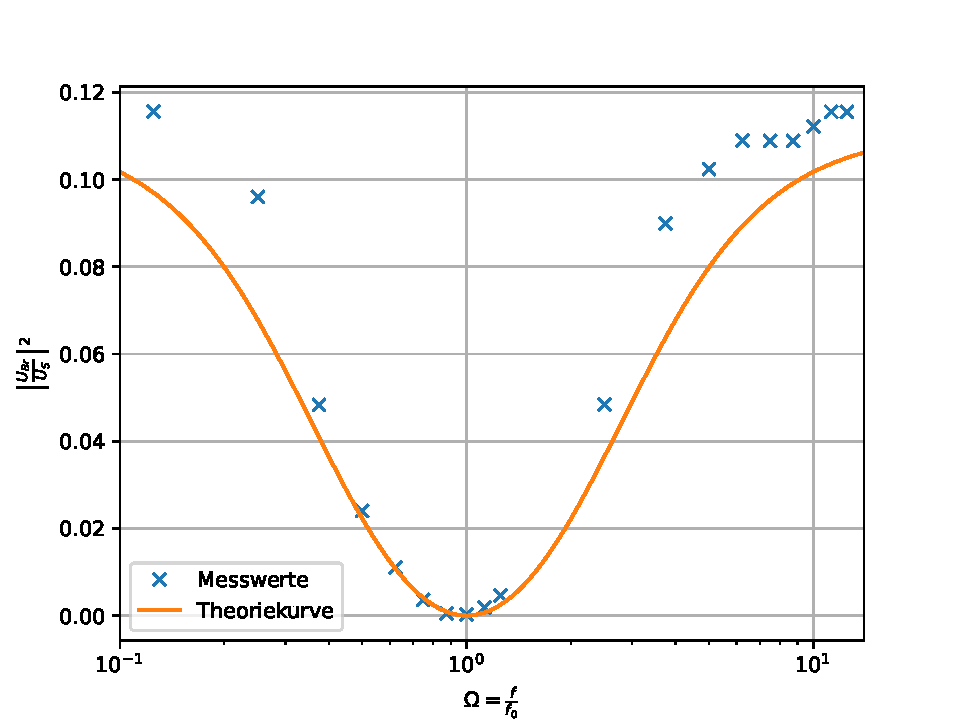
\includegraphics[width=0.95\textwidth]{plot.pdf}
  \caption{Halblogarithmische Darstellung der Frequenz und Spannungen.}
  \label{fig:WienRobinson}
\end{figure}
Der Klirrfaktor wird mit der Gleichung (\ref{eqn:}) bestimmt. Allerdings wird die Summe der Oberwellen mit der zweiten Oberwelle angenähert.
Die zweite Oberwelle $U_2$ bestimmt sich aus der Gleichung (\ref{eqn:}) und durch
$$U_2 = \frac{U_{\text{Br}}}{f(\Omega = 2)}\,,$$
wobei für $U_{\text{Br}}$ die minimale Brückenspannung verwendet wird. Somit ergibt sich 
$$U_2 = \frac{15\unit{\milli\volt}}{\sqrt{\frac{1}{45}}} \approx 100,62\,\unit{\milli\volt}\,.$$
Daraus bestimmt sich der Klirrfaktor
$$k = \frac{U_2}{U_1} = \frac{U_2}{U_{\text{S}}}= \frac{100,62 \cdot 10^{-3}\,\unit{\volt}}{1\,\unit{\volt}} = 0,10\,.$$